\documentclass[onecolumn, draftclsnofoot,10pt, compsoc]{IEEEtran}
\usepackage{graphicx}
\usepackage{url}
%\usepackage{setspace}

\usepackage{geometry}
\geometry{textheight=9.5in, textwidth=7in}


% 1. Fill in these details
\def \CapstoneTeamName{			Addax}
\def \CapstoneTeamNumber{		38}
\def \GroupMemberOne{			Caitlyn Cook}
\def \GroupMemberTwo{			Iliana Javier}
\def \GroupMemberThree{			Nicholas Skinner}
\def \GroupMemberFour{			Amy Tang}
\def \CapstoneProjectName{		Impala performance tuning on HDFS}
\def \CapstoneSponsorCompany{	Hewlett Packard}
\def \CapstoneSponsorPerson{	Andy Weiss}

% 2. Uncomment the appropriate line below so that the document type works
\def \DocType{		Project Update Winter 2019
				%Research Proposal Document
				%Technology Review
				%Design Document
				%Progress Report
				}
			
\newcommand{\NameSigPair}[1]{\par
\makebox[2.75in][r]{#1} \hfil 	\makebox[3.25in]{\makebox[2.25in]{\hrulefill} \hfill		\makebox[.75in]{\hrulefill}}
\par\vspace{-12pt} \textit{\tiny\noindent
\makebox[2.75in]{} \hfil		\makebox[3.25in]{\makebox[2.25in][r]{Signature} \hfill	\makebox[.75in][r]{Date}}}}
% 3. If the document is not to be signed, uncomment the RENEWcommand below
%\renewcommand{\NameSigPair}[1]{#1}

%%%%%%%%%%%%%%%%%%%%%%%%%%%%%%%%%%%%%%%
\begin{document}
\begin{titlepage}
    \pagenumbering{gobble}
    %\begin{singlespace}s
    	\includegraphics[height=4cm]{coe_v_spot1}
        \hfill 
        % 4. If you have a logo, use this includegraphics command to put it on the coversheet.
        %\includegraphics[height=4cm]{CompanyLogo}   
        \par\vspace{.2in}
        \centering
        \scshape{
            \huge CS Capstone \DocType \par
            {\large\today}\par
            \vspace{.5in}
            \textbf{\Huge\CapstoneProjectName}\par
            \vfill
            {\large Prepared for}\par
            \Huge \CapstoneSponsorCompany\par
            \vspace{5pt}
            {\Large\NameSigPair{\CapstoneSponsorPerson}\par}
            {\large Prepared by }\par
            Group\CapstoneTeamNumber\par
            % 5. comment out the line below this one if you do not wish to name your team
            \CapstoneTeamName\par 
            \vspace{5pt}
            {\Large
                \NameSigPair{\GroupMemberOne}\par
                \NameSigPair{\GroupMemberTwo}\par
                \NameSigPair{\GroupMemberThree}\par
                \NameSigPair{\GroupMemberFour}\par
            }
            \vspace{20pt}
        }
        \begin{abstract}
        % 6. Fill in your abstract    
            The Big Data team at Hewlett Packard currently uses an Oracle database to store industrial IoT data gathered from large printing presses. 
            They are interested in moving from their current centralized database to a distributed architecture, and have asked our team to investigate the operation of their planned system.
            This report introduces our project, defines our goals, discusses the work completed during Fall and Winter Terms, and discusses some challenges encountered during Winter term.
        \end{abstract}     
    %\end{singlespace}
\end{titlepage}
\newpage
\pagenumbering{arabic}
\tableofcontents
% 7. uncomment this (if applicable). Consider adding a page break.
%\listoffigures
%\listoftables
\clearpage

% 8. now you write!
\section{Project Description}
\subsection{Background}
The HP BackOffice database stores data collected from approximately 300 industrial printers, called web presses, in operation globally.
The presses print on paper up to 110 in wide at the largest, and are capable of printing at speeds of up to 1000 ft per minute in full color.
The presses are used to print books, packaging, and mail at an industrial scale for many major companies.
For example, the presses are a part of how Amazon is able to print and ship a brand new copy of a book within 4 hours of ordering it on their website.

Each press records data that is used to diagnose issues, study press operation, and guide the development of new features.
Data is collected on alarms, pen health, print jobs, and other aspects of operations.
This data is streamed to HP's database, where it is processed and analyzed by teams of engineers.
New data is added to the database at a rate of approximately 60 - 100 GB per day; currently, the database holds approximately 30TB of data. 

HP's current database is a centralized Oracle 12c database which shares all memory and disk resources between multiple processors.
While Oracle databases handle transactions extremely well, HP doesn't have much need for transactions. 
Their data is static once written; once the data for a day is collected and stored, it is not further modified.
Instead, HP mostly performs analytic processing on their data, which suffers unnecessarily from the overhead that makes Oracle so good at transactions.
The monolithic architecture of their current database also presents difficulties with scaling.
As HP anticipates future data loads, they want a solution that will allow cheaper and more efficient scaling.
This is their motivation behind our project; we are to investigate the behavior of a distributed system which will fare better in these key areas.
Our research will result in information that will help ease their transition process.

\subsection{Purpose}
HP's data team has tasked us with gathering information about a distributed database system implementation. 
The data team is particularly interested in Apache / Cloudera Impala, a SQL engine that runs on the popular Hadoop Distributed File System (HDFS), and would like us to focus on researching this engine's mechanisms. 

Our sponsor has a variety of reasons for being interested in distributed database systems.
At the core of every business and engineering decision is cost, in terms of both time and money.
In terms of time, HP's current exponentially growing database is causing queries to result in long running times.
This is due simply to the large amount of data tables that need to be scanned, reduced, or joined by the single server.
In addition, there is significant slowdown caused by the overhead Oracle implements for each query.
This work could be eased by implementing a system that distributes queries across multiple servers.
HP has also spent years understanding and optimizing their SQL queries to best fit their data's behavior, so they would like any new system they adopt to run SQL as well.
Apache Impala fits these criteria.
Monetarily, HP is interested in moving to an open source solution to cut the cost of Oracle's software licensing fees, which grow more expensive the more data the database houses.
Impala, as well as its underlying Hadoop system, is open source. 
These criteria make Impala a promising solution for HP's data problems.

\subsection{Goals}
The goal of our project is to produce a document that will guide a person familiar with shared-everything database architectures through the setup and use of a shared-nothing architecture.
We will focus on multiple aspects of the system and provide an explanation of their function which will allow the reader to examine and improve the performance of a distributed system.
In particular, this document will examine the tools available for diagnosing and tuning performance problems, the metadata store of the database, the generation of query plans and how parallelization across nodes affects these plans.
We will accomplish this through a combination of experimentation and reading existing documentation.

\subsection{Challenges}
Last term, we had the challenge of defining our own assignments.
This term, we have taken one of the assignments produced last term and expanded it to fulfill the requirements of our final deliverable for HP.
Modifying the existing document has produced some challenges, as our audience for the paper has shifted from Capstone graders to HP’s team.
We have also encountered some difficulty answering questions we intended to write about that were not explicitly addressed by documentation or other research.
To answer these questions, we have had to broaden the scope of our search as well as do some experimentation of our own. 

We have also been challenged this term to represent our project in accessible terms, through both a poster and elevator pitches.
Our project has proven difficult to explain in simple terms, as it doesn’t involve many pieces of well-known technology that provide a good hook to interest the public.
Through collaboration with our client and feedback from our poster critique, we have generated ideas for poster content, graphics, and discussion points that we hope will address this challenge.

\section{Fall Term Work}

Once assignments were defined, we begun work by reviewing a selection of relevant papers suggested by our client. 
The first four of the papers discussed below were the subject of a more detailed analysis and write-up, while the others were used as supplementary sources for an additional assignment. 
All papers discussed can be found in the bibliography at the end of the report.
Below the review of this reading is a week-by-week summary of our progress throughout the term.

\subsection{Review of Papers}

\subsubsection{E. F. Codd - A Relational Model of Data for Large Shared Data Banks}

To begin our reading, our client suggested "A Relational Model of Data for Large Shared Data Banks" by E. F. Codd.
Published in June of 1970 in the Communications of the ACM, the paper forms the foundation for relational databases that are in use nearly everywhere today.
Codd was concerned with insulating the user from changes in the structure of data storage, which he felt that the user should not need to be aware of.
To accomplish this, Codd outlines an application of set and relation theory to databases. 
The concept of normalization is introduced, including normal form and associated concepts such as primary and foreign keys.
Once he has established the concept of normal form, Codd discusses operations and interactions with the table that form the basis for database languages, including SQL. 

\subsubsection{The Oracle Optimizer: Explain the Explain Plan}
To recommend changes, our team needs knowledge of the current system. 
Our team will be researching and comparing two different systems, but to begin, we require a point of reference.
To understand the Oracle 12c system currently in use, HP has recommended reading  "The Oracle Optimizer: Explain the Explain Plan" guide.
The Oracle Optimizer is a tool that attempts to resolve the most efficient execution plan for a given query using histogram information in addition to data projection based on indices and dependencies.
The optimizer aims to reduce the time and CPU usage to resolve the query.
To aid the user in understanding its actions, the Oracle Optimizer can generate a log of the execution plan of a query  to display to the user.
Logs generated by the optimizer also include information on the resources used to accomplish the task.
An execution plan is referred to as an Explain Plan. 
An Explain Plan from the Query Coordinator takes relevant information about the table structure and dependencies from an executable query and compiles the metadata needed to generate an efficient plan to execute the operation.
The Query Coordinator takes in (1) how much CPU is available, (2) the projected time to dispatch and complete individual operations, (3) the composition of the query and (4) external dependencies on the involved tables.
With these inputs, the Query Coordinator forms an educated estimation of what methods and what order it should execute the query.

The "Explain the Explain Plan" paper is a thorough, yet concise resource on Oracle's Query Coordinator.
The paper goes through detailed information on query planning and coordinating, measuring the weights of different actions and comparing them against the current value of available resources.
Cardinality, access methods, join methods, join types, join orders, partition pruning and parallel execution are all vital components to query optimization that will change the cost of a query plan.  

\subsubsection{Dremel: Interactive Analysis of Web-Scale Datasets}

This paper provides fundamental concepts of Dremel, from its architecture to implementation, and explains how Dremel makes more efficient performance than MapReduce computing does.
Data in Dremel is organized in a "columnar" format, which contributes to very fast query speed.

Dremel is a distributed system for interactive analysis of large datasets. It is also a custom, scalable data management solution built from simpler components. Dremel complements the MapReduce paradigm, and provides fault tolerant execution just like MapReduce does.
It also includes a flexible data model and in situ data processing capabilities.
In situ refers to the ability to access data 'in place'. 

Importantly, Dremel uses a columnar nested storage.
The architecture of Dremel has the same concept of a serving tree used in distributed search engines.
The query gets pushed down the tree and is rewritten at each step. 
The result of the query is assembled by aggregating the replies received from lower levels of the tree.
Dremel supports a SQL-like syntax, but does not support update or create functions. 
In contrast to layers such as Pig and Hive, it executes queries natively without translating them into MapReduce jobs.
Besides, Dremel uses a column-striped storage representation. 
The data is represented as a set of columns. 
The advantage this brings is that it allows users to read less data by retrieving only columns they need, which reduces CPU cost.

Based on the major idea of the project is focusing on switching to distributed system, this paper helps us to have a comprehensive understanding of distributed system that uses columnar nested storage, and clarifies differences between row storage and columnar storage.

\subsubsection{Impala: A Modern, Open-Source SQL Engine for Hadoop}

This paper served as an introduction to the rest of our research going forward. 
Impala is an open source SQL engine designed to run with high concurrency and low latency on distributed frameworks such as Hadoop.
This paper detailed Impala's SQL engine, while also detailing how it works as a distributed framework- specifically how it distributes data and queries over the Hadoop Distributed File System.
This paper gave some explanation from a user's point of view, such as how to create a table and where in the file system that data would be stored. 
However, most of the paper detailed Impala's architecture: its frontend code, backend code, and data storage. 
The Impala front end is where the SQL is translated into execution plans, and the backend is where these plans are actually carried out.
Query plans in Impala's front end have two stages: single node planning, and plan parallelization and fragmentation-- to prepare the query for distribution across all of the system's nodes. 
When the query plan is optimized, "cost estimation is based on table/partition cardinalities plus distinct value counts for each column".
The second part of the frontend planning has two goals for plan distribution: to minimize the amount of data movement and to maximize "scan locality". 
These two terms which are related, and are placed at such high importance due to the Hadoop File System remote reads (reads not from the current node) being much slower than local (all data found within the node) ones.
Impala's backend, the query executor, runs on each node in the system independently.
This backend also manages I/O and storage formats.
The paper also pointed out the roadmap for where the Impala developers wanted it to be in the future, which also conveniently highlighted certain standard SQL and database features that Impala is currently missing. 

This paper served as a starting point for where our research for the rest of the term will go. 
The questions posed in our project goals were touched on briefly in this paper, but none were discussed in the amount of depth required for our sponsor’s needs.
However, this paper did give us indications for where we can go to find the information needed to answer our questions, such as how we can investigate Impala’s frontend more to learn about its query planning, and how we can read more about the backend to learn more about how it handles distributions. 

\subsubsection{Parallel Execution with Oracle Database 18c Fundamentals}

Oracle is an example of a database system that implements shared-everything architecture.
The data contained within the Oracle system is accessible to all processing units without limitations. 
The parallelism implemented within the Oracle system is not limited to the data access that an individual node would possess.
Rather, all dispatchable agents associated with the database are capable of accessing all the data contents.

Oracle's shared-everything architecture does not require data partitioning to enable parallelism by default; data is accessible from all processing units without limitations.
Parallelism within the Oracle system is implemented through dividing a query into smaller components called granules.
Granules represent a fraction of a query, and can be assigned a specific block range in memory.
These block-based granules are assigned a position within the memory or storage of the Oracle system, and will do all actions within their block range.
Upon resolving a task, a granule will need to report its result set to another agent.
The action it will take to complete this task is known as 'data redistribution', and it is a key component to many non-trivial parallel operations, including parallel aggregations, joins and sorts. 
The individual granule does not know the broader context of the operation the retrieved data will be used within, so it must pass the result set to a subsequent operation on the result set contents.
The query coordinator will dispatch an agent to grab the result set from the previous granule, and assign the new agent a granule of work to process. 
This series of events is recursively performed until the end query result is reached.

The manual is an additional resource that will be used going into the team's research. 
The manual presents a fundamental explanation of Oracle's implementation of the shared everything architecture. 
The manual covers basics of how memory and processing are shared between agents through to the extensions of the Oracle program to accommodate shared-nothing methodologies.
It also contains information regarding Oracle's attempt to address the benefits within the shared nothing architecture.
Partition based granules are an example of approaching the distributed nodes with dedicated agents within oracle. 

\subsubsection{The Case for Shared Nothing}
"The Case for Shared Nothing" by Michael Stonebraker is a short paper that vaguely describes the merits of shared-nothing architectures.
He provides a simple table which ranks shared-nothing, shared-memory, and shared-disk architectures based on performance in terms of "difficulty of concurrency control", "number of messages", and other vague criteria.
Several of these criteria are not well defined, and none define clearly how Stonebraker came to his conclusions regarding the rankings the assigned.
Although this paper was quite vague, it introduced us to criteria we can use to compare shared-nothing and shared-everything architectures, which our sponsor is very interested in learning the benefits and faults of. 

\subsection{Weekly Progress}
\begin{tabular}{l | p{5 cm} | p{6 cm}  | p{5 cm} }
    Week & Details & Problem \& Solution & Assignment Due \\ \hline
    Week 3 & We were assigned to groups. We set up the Slack channel and Github repo. We had our first meeting with the client to get details for problem statements, and scheduled future meetings with our client and TA.& & Problem statement - individual \\
    Week 4 & We had another meeting with our client to discuss the project in more detail.& & Problem statement - group final \\
    Week 5 & We decided on choosing the Research Proposal over the Requirements Document, and assigned sections to complete.& Problem: We had difficulty brainstorming on how to write a paper that is helpful to our project, and needed more direction. Solution: We met with Dr. Winter, who modeled our writing assignments. We also set up weekly meetings with her.& \\
    Week 6 & We clarified understanding of paper contents with our client and instructor. & Problem: Dr. Winters was concerned about the white paper literature review being either too ambitious a project or not satisfying the term's requirements. Solution: We discussed with her and our client how the aassignment could be modified to meet the requirements within our timeframe.& \\
    Week 7 & Dr. Winters gave feedback on our draft Research Proposal, and we planned the small-scale literature review. & & Research Proposal \\
    Week 8 & We met and discussed the contents of the chosen 4 papers with our clients, and began work on the review paper.& & \\
    Week 9 & Dr. Winters and our clients spoke directly, and clarified the assignments for the term. We received permission to stop meeting with our TA and meet with Dr. Winters instead.& & Review paper\\
    Week 10 & We dividied sections for the systems comparison paper. & & \\
    Week 11 & Finals week & & Group system comparison paper, Progress update video and report \\
\end{tabular}
\section{Winter Term Work}
\subsection{Project Status}

Work this term has been divided roughly into two sections.
The first half of the term was spent researching various topics through Impala documentation, source code, and other independent sources.
The later part of the term has been focused on compiling the understanding gained from this research into a paper that will be our final deliverable.
The outline of this paper is given below; summaries of the sections that have been addressed at this time are given in the Research Focus section.

\begin{figure}[ht]
    \centering
    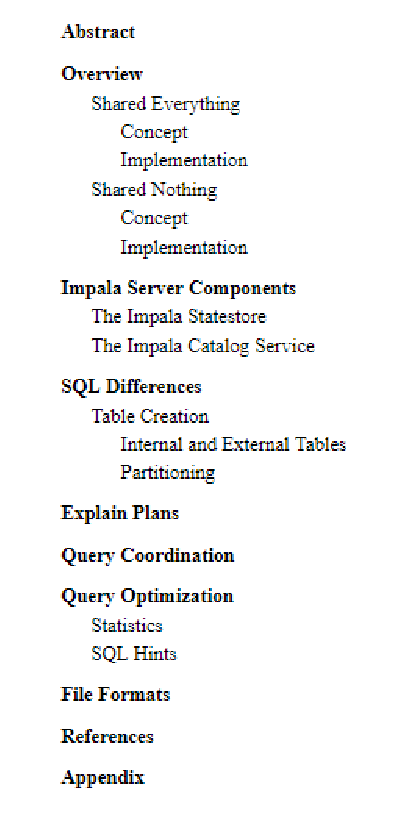
\includegraphics[width=\linewidth, height=4in, keepaspectratio]{ToC.eps}
\end{figure}

\subsection{Research Focus}
\subsubsection{Apache Impala Guide}
Throughout the term, we have been referring to Cloudera’s latest documentation for Apache Impala to research Impala’s inner workings.
The Apache Impala Guide is a comprehensive guide to every topic related to Impala, from installation and architecture to administration and optimization.
It is approximately 770 pages, which means it contains more detail than is necessary for engineers at HP to start working with the system.
It is also not specifically tailored towards engineers moving from an Oracle system to Impala, which is what HP’s engineers are doing.
While it is a good comprehensive guide filled with many fine details about the structure and operation of Impala, it is still missing some important information, such as details about the Statestore daemon, which our team had to look elsewhere to find information on. 
\subsubsection{Impala Server Components}
Impala is bundled with services that assist the Hadoop Distributed File System.
The services within the Impala ecosystem are intended to increase the overall performance of query execution through coordination between impala nodes.
Impala also possesses a number of optional services, which help to produce and optimize components of the service.
The two predominant services are the Statestore and the Impala Catalog Service. 

The Impala Statestore is a mandatory service for the Impala distributed system.
It must be running at all times, and if it is not, queries that involve nodes other than the initiator will not be able to resolve.
The Statestore acts as an arbitrator of the system, giving each node the information it needs to resolve a query, as well as keeping each individual node up to date with the most recent data commits.
Impala also uses the Statestore as a lexicon to interface with the other services that assist in improving impala’s performance, one of those services being the Impala Catalog Service. 

Impala’s Catalog Service is a daemon that is focused on the collection and update of metadata.
Metadata is collected from each node, and is placed into a central repository called the Metastore, which is shared within the service.
In application, the service acts as a listener for any DDL/DML changes within the Impala system.
When the Catalog Service detects a change, it grabs the new information and interfaces with the statestore to update the Metastore.
The service is a non-vital portion of the Impala ecosystem, and as such is an optional tool.
Its effects can be replicated by appending a REFRESH command after every SQL commit.

\subsubsection{SQL Differences}
The type of SQL used by Impala is known as HiveQL; while it conforms to the 2016 ANSI SQL standard, there are differences between the SQL currently used by the BackOffice team and HiveQL.
This section of the document is intended to point out areas where those changes may produce confusion or difficulty when transitioning.

A notable entry in this section are changes in the method of partitioning.
Oracle allows three methods of partitioning large tables: value, range, and hash partitioning.
However, Impala allows only value partitioning.
Methods for simulating the disallowed partition strategies are discussed, and syntax for implementing partitions is given. 

Also discussed in this section are the Impala definitions of internal and external tables.
Oracle also makes use of internal and external tables, but in a more limited fashion than Impala.
The methods for creating both kinds of tables are discussed, as well as the management of the files during updates, inserts, deletes, and drops. 

Planned additions to this section are a discussion of analytic functions, which are heavily used by HP when handling their data.
This section will seek to identify functions that are supported in Oracle’s SQL but not in HiveQL, as well as any differences in syntax or behavior across versions. 

\subsubsection{File Formats}
In this term, we looked into several file formats that used in Apache Hadoop, which are Avro, Parquet and Optimized Row Columnar (ORC).
Each of these file formats is unique and has their own relative advantages and disadvantages.
It is important to choose file format used in Impala table since file format has significant impacts on the performance.
For example, some file formats enable compression that may affect size of data and consequently lead to I/O and CPU resources required to deserialize data.
 
Parquet and ORC are column based file format, and Avro is row major file format.
We found that Parquet is a good choice when you need to query a specific column with wide table, or work on some aggregation operations such as SUM() and AVG() that need to process most of the values in a column.
Parquet table can also minimize I/O by reading less data and retrieve values from column quickly.
 
ORC is an optimized version of RCFile.
However, Impala does not support it.
It makes improvement on the compression by using an encoder that handle different column data types.
ORC also skips blocks of rows that are not needed in query and then indexing fewer files and reduce load.
This is why ORC has the better compression than Avro and Parquet.
 
Avro is a row major file format.
Impala can query and create Avro tables, but not insert them. 
Avro schemas are defined with JSON and so it stores data definition in JSON after creating Avro tables. 
Currently, Avro tables do not support TIMESTAMP columns, but there are two functions that help to store time values. 
For some reason, mismatch of values type may occured between Avro schema and column definition in the database.
To solve this problem, Impala uses schema reconciliation to check mismatching number of columns.

\subsubsection{Query Optimization}
Through this term, we discovered that most query optimization hinges on the statistics of the data being queried.
The number of rows in a dataset is particularly important, as this directly shows how much data needs to be processed.
The amount of data to be processed, along with other  affects the type of JOIN operation Impala’s internal query optimizer uses in the query processing.
An incorrectly chosen JOIN operation can result in a query taking much longer than it should to be processed. 

Several commands exist to compute and modify data table statistics. The simplest of these commands is the COMPUTE STATS [Table\_Name] command. 

An engineer can manually change table statistics to influence the query optimizer’s choices.
An engineer can also include SQL hints within their queries to influence the query optimizer.
Such hints are also available in Oracle systems, and the differences between the two systems’ SQL hint coverage is discussed in this section.  

\subsection{Weekly Progress}
\begin{tabular}{l | p{15 cm}}
    Week & Details  \\ \hline
    Week 1 & During Week 1, we scheduled meeting times with our client, and had our first interactions with an Impala test environment. We discussed research topics for the term, and planned our initial topics. \\
    Week 2 & We discussed our initial research topics, and discussed the change in Impala interface. An HP employee has donated use of a server in their home to run a single-node Impala instance. This will allow us to use and investigate Impala without concern for cost. Our previous alternative was AWS, which requires paying for all server uptime. We discussed our elevator pitches, as well as our research for the week, including the catalogd daemon. \\
    Week 3 & Our client meeting this week was cancelled due to our client having car troubles, resulting in them being unable to make it. We rescheduled the meeting for Monday of next week. In the meantime, we investigated various related Hadoop components, and continued investigation of the catalogd daemon. \\
    Week 4 & We had two meetings this week to make up for the missed meeting in the previous week. We investigate partitioning, file formats, the statestored and catalogd. We set a goal of having an outline of the system comparison paper for our next meeting, to begin writing and review of our final document. \\
    Week 5 & Nate and Andy gave us some help with our difficulties inserting images into the .tex file of our document. We resolved the issue by converting the images to .eps files. We reviewed the outline and section headings of our final paper, as well as elevator pitch drafts and poster ideas. We have had some difficulty coordinating the poster review, but it was scheduled for the following week.  \\
    Week 6 & Nathaniel Whitlock reviewed parts of our rough draft for our final paper. During this work meeting we researched into SQL differences and query optimization to better fill out those sections in the paper. Nathaniel also clarified our questions in regard to the paper’s audience and purpose, and so we planned to tailor the paper more towards HP’s engineers, who have some background on SQL and relational databases, and are coming from a background of working with Oracle systems. We also took part in the initial poster critiques with team 67. Both teams gave insightful and helpful comments on each other’s posters and we came out of the meeting with more ideas for what needs to be on our poster.  \\
    Week 7 & We reviewed our rough (alpha) draft of our final paper with Andy Weiss and Nathaniel Whitlock. They made suggestions, corrections, and answered our questions as they read through the paper. In particular, Andy was able to find a more detailed price range for the new system that we could use to demonstrate its cost efficiency when presenting to the public. Going forward we will follow their suggestions to fix inconsistencies and expand on certain sections.  \\
    Week 8 & We reviewed the status of the paper, including the new changes since the previous week filling in sections that were identified as currently lacking. We addressed specific comments provided by Nate and Andy, and standardized some terminology across sections and authors. \\
    Week 9 & We discussed the addition of the last new sections to be added. We reviewed the sections on manual metadata manipulation and analytic functions with Nate and Andy and discussed possible reorganizations for the document. Our meetings with the client and with professor were both cancelled. \\
    Week 10 & We worked individually on filling out our sections of the paper and getting further clarification on details from Nate and Andy. We began work on our end of the term progress report and video. No meetings with client or Dr. Winters this week. \\
\end{tabular}

\subsection{Individual Contributions}
Please note that formatting may not be properly in place for this section, due to limitations on the number of subheadings in LaTeX.
\subsubsection{Nicholas Skinner}
Impala Server Components

The Impala Statestore

The Impala Statestore broadcasts service messages to each node in the cluster.
This is done to gain an understanding of the current state of the cluster, and any modifications that may need to be made.
The messages that are broadcasted come in two distinct forms: Heartbeats, and Topic Updates.
These message types contain information the Statestore requires to determine what actions it needs to take. 

A Heartbeat within the HDFS is an interaction between a datanode, and its namenode intended to indicate presence.
The heartbeat exists as a keepalive message to ensure that the datanode is still working within the cluster.
After a user specified interval, if a number of heartbeats have not been received from the datanode, the namenode will consider the datanode to be out of service. 
Blocks hosted by the out of service node will be marked as unavailable until the datanode is able to become active, or replicas of the available data blocks are created on other nodes.

A Topic Update within the HDFS is a message containing information on new developments regarding a topic.
The Topic update message will send and receive information from subscribers to specific topics. 
An individual node is able to subscribe to modifications of topics of interest at start-up by providing a list of their topics of interest. 
Subscribers of a specific topic will receive information on new entries, modified entries, and deletions. 
If an individual node makes a change to a topic, it must wait for the Statestore to broadcast a new topic update before other nodes are able to receive the new modifications. 

Statestore Command Line Arguments:

The Impala Statestore possesses command line arguments that may alter the number of process threads dedicated to its service as well as the frequency that update messages or heartbeats are sent to the associated nodes.
These arguments are to be appended to the command line startup.
A command to start the Impala Statestore should look similar to the following statement:
\begin{center}
\begin{tabular}{ |c| }
    \hline
    \$ sudo service impala-state-store start \\
    \hline
\end{tabular}
\end{center}

If a restart is required, the following command should be used:

\begin{center}
\begin{tabular}{ |c| }
    \hline
    \$ sudo service impala-state-store restart \\
    \hline
\end{tabular}
\end{center}

Statestore Number of Threads

\begin{center}
\begin{tabular}{ |c| }
    \hline
    \$ -statestore\_num\_update\_threads 10 \\
    \hline
\end{tabular}
\end{center}

This command will modify the current number of threads that are dedicated to sending topic updates.
Impala suggests to keep this at its default value of 10.

Statestore Update Frequency

\begin{center}
\begin{tabular}{ |c| }
    \hline
    \$ -statestore\_update\_frequency\_ms 2000 \\
    \hline
\end{tabular}
\end{center}

The frequency, designated in milliseconds, that the Statestore attempts to send a Topic Update to each subscriber.
By default Topic Updates occur every 2000 milliseconds (2 seconds).

Heartbeat Number of Threads
\begin{center}
\begin{tabular}{ |c| }
    \hline
    \$ -statestore\_num\_heartbeat\_threads 10 \\
    \hline
\end{tabular}
\end{center}

This command will modify the number of threads that are dedicated to sending heartbeats.
Impala claims that it is non-typical to modify this value 10.

Heartbeat Frequency

\begin{center}
\begin{tabular}{ |c| }
    \hline
    \$ -statestore\_heartbeat\_frequency\_ms 2000 \\
    \hline
\end{tabular}
\end{center}

The frequency, designated in milliseconds, that the Statestore attempts to send a heartbeat to each subscriber.
By default heartbeat messages occur every 1000 milliseconds (1 second).
Impala claims that this value should be capable of supporting catalogs and clusters up to 150 nodes, beyond that you may be required to increase the heartbeat delay.



The Impala Catalog Service

The Impala Catalog Service is a component of the Impala server that relays metadata changes from Impala DDL and DML statements.
This catalog service is physically represented by a daemon process ‘catalogd’ which interfaces with the Statestore component to collect metadata changes for each Impala node.
Metadata changes are then collected into a unified database named the ‘Metastore’, which is intended to create a metadata directory to assist query resolution speeds. 
The Impala Catalog Service exists to minimize need for manual refreshes of metadata store (The SQL commands REFRESH and INVALIDATE METADATA are still valid if not changing any DDL/DML directly). 
Updates to the metastore performed by the catalogd daemon are performed every topic update. 

Even with automatic metastore updates, the Impala Catalog Service is unable to detect new information and modifications to the dataset from specific methods of interfacing with the Impala ecosystem.
The following actions will not cause a Metastore update:

\begin{itemize}
    \item DDL/DML statements done through HIVE.
    \item Manipulating data files directly within the HDFS.
    \item Any non-DDL/DML statement changes to the dataset.
\end{itemize}

In these instances, the Catalog Service is unable to detect changes within the system, and is unable to force a refresh on the Metastore.
To resolve this, a manual refresh command must be executed against at least one node.

Because requests by the catalogd daemon are passed through the Statestore daemon, it is recommended to run both services on the same host. This will reduce the network communication required between the systems.

The catalogd daemon is a non-critical service, meaning it does not need to be active at all times.
When an error prevents the catalogd service from carrying an action, no data loss occurs, though the metastore may not possess the latest metadata from each node. 
If the daemon has not been run for an extended period, and a REFRESH command has not been executed, the data possessed by the metastore will be out of date, but is still accessible by virtue of being hosted through the statestore.

Catalog Service Command Line Arguments:

The catalog daemon comes with a select few arguments that can control how the service loads metadata. The service itself can be started by issuing the host machine the following command:
\begin{center}
\begin{tabular}{ |c| }
    \hline
    \$ sudo service impala-catalog start \\
    \hline
\end{tabular}
\end{center}

If a restart is required, the user is able to simply use the following command:

\begin{center}
\begin{tabular}{ |c| }
    \hline
    \$ sudo service impala-catalog restart \\
    \hline
\end{tabular}
\end{center}

Load In Background:

The Catalog Service provides an argument option to either load all metadata before accepting a request, or asynchronously load data to enable sending requests as soon as the service is started.
Asynchronous loading is the current default option in Impala, however, the other method can be enacted through the following argument:

\begin{center}
\begin{tabular}{ |c| }
    \hline
    \$ --load\_catalog\_in\_background=false \\
    \hline
\end{tabular}
\end{center}
The Metastore

Impala keeps table definitions for each node within a centralized traditional database called the metastore.
Impala also tracks additional metadata for the low-level characteristics of data files, including the physical locations of blocks within HDFS.
Each Impala node caches all of this metadata to reuse for future queries against the same table. 
The metastore collects metadata from each node in a cluster, and shares this collected data with all the nodes in the cluster.

Metadata within the HDFS is capable of being automatically updated through the catalogd daemon if the modifications are limited to a DDL or a DML change. 
The catalogd daemon relays the metadata changes from Impala SQL statements to all the Impala daemons in a cluster.
For more information about the catalogd daemon, refer to the Impala Catalog Service section. 
 
When needed, a manual metadata refresh can be performed by executing either the INVALIDATE METADATA or the REFRESH commands on a specified table.
INVALIDATE METADATA [table\_name] will reload all metadata for the specified table, updating all facets of the system’s understanding of the current metadata composition.
The REFRESH [table\_name] command will only update the metadata of the table with the locations of newly added blocks.
REFRESH allows a lightweight update of the system, but if more extensive changes have been made, it is recommended to use INVALIDATE METADATA to avoid performance degradation.
If a metadata update of the entire system is required, it can be performed by using INVALIDATE METADATA with no table suffix.
This will cause the Impala system to tag each node to re-create metadata for all tables.

\subsubsection{Caitlyn Cook}

Query Coordination

When a query is submitted to Impala, the node that receives it takes on the role of Query Coordinator (QC).
Any node can take on this role, and multiple nodes can be performing this role simultaneously for different queries.
Once a node takes on the role of QC for the query, it assigns work to known active nodes, including itself. 
All nodes complete their work on the data that they have, and return their results to the coordinating node, which compiles them and returns the information to the user. 

When possible, work is assigned so that data does not need to be transmitted from node to node. 
Instead, the nodes holding that data are assigned the work needed to be done. 
This improves execution time by taking advantage of data locality. 
However, it is not always possible to execute in this way; for example, in the case of some joins, some table data must be transmitted between nodes. 

While it is a supposed advantage to distributed systems that there is no single point of failure, it is important to note that only one node runs the statestored and catalogd. 
Queries will not automatically fail should they be received while the node with these processes is down, but they will continue to work with outdated information, which may have negative consequences. 
For more information on these processes, see the Impala Server Components section. 

\begin{figure}[ht]
    \centering
    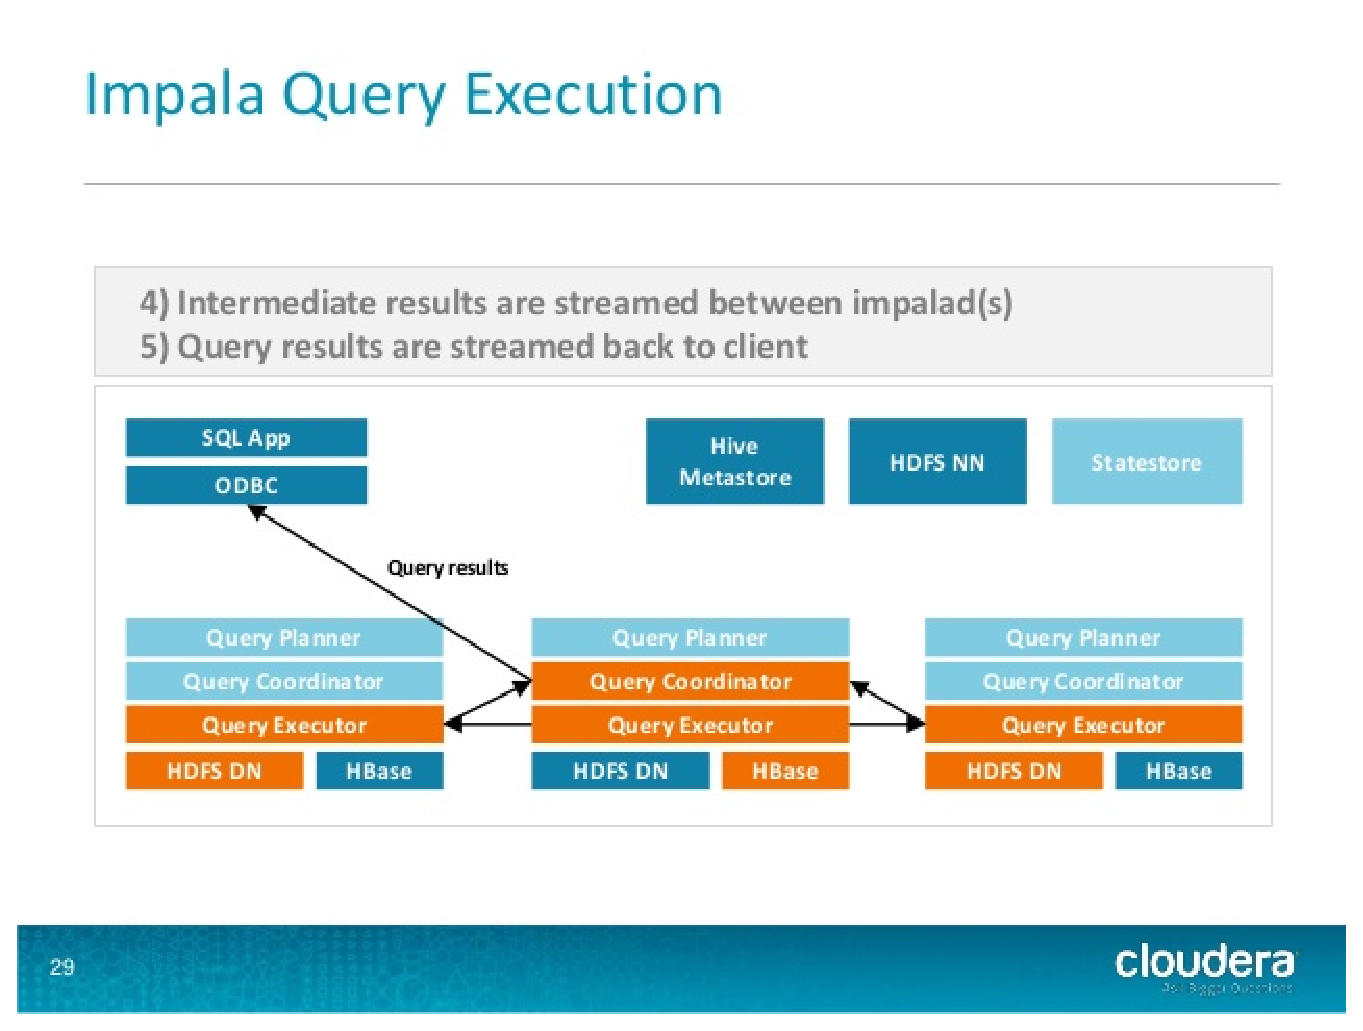
\includegraphics[width=\linewidth, height=4in, keepaspectratio]{qc.eps}
\end{figure}

While the default behavior is for all nodes to act as both coordinator and executor when needed, it is possible to configure Impala with dedicated coordinator nodes.
This can reduce the amount of network traffic by reducing the amount of communication with the statestored required, as only the coordinating nodes need to be aware of the status of all other nodes.
This can be useful when there is a large volume of highly concurrent queries, which generate a large volume of traffic.
If this option is chosen, it is recommended that there is about 1 dedicated coordinator for every 50 dedicated executors. 
\newline
SQL Differences


HiveQL conforms to the 2016 ANSI SQL standard. 
Most behaviors are similar or identical between Oracle and HiveQL, but notable differences are discussed below. 

Table Creation

Internal and External Tables

To create a table, use the CREATE TABLE statement. 
By default, an internal table is created; an external table can be created by adding EXTERNAL to the statement. 

When an internal table is created, Impala creates the necessary directory to hold the data in the default Impala workspace. 
Data is then added to the table after creation using the INSERT or LOAD DATA statements. 
If the table is renamed, Impala will move the files to a directory with the new name, even if the files were originally located outside of its workspace. 
If the table is dropped, Impala will delete all data files in the table. 

By contrast, an external table’s files are not directly managed by Impala. 
When creating an external table you should supply a LOCATION statement that tells Impala where the files are stored. 
If you do not supply a location, Impala will use the default location, as if it were an internal table, but will still not manage the files. 
Impala will treat any files in this location as part of the table, and new data can be added through INSERT or LOAD DATA statements as with internal tables. 
If the table is renamed or dropped, Impala will not modify the files at all, since it is not managing them. 
Dropping the table will remove Impala’s association with it, but they may continue to be used by other Hadoop or HDFS components.
Otherwise, an external is the same as an internal table. 
It can contain any file type, and will behave the same as an internal table.

Alternatively to creating a table and loading/inserting data, you can use a CREATE TABLE AS SELECT statement.
In this case, omit the column definitions at the top of the statement, and add a SELECT statement beneath all options. 
You may also choose to omit column definitions if you are loading a Parquet file, as they may be inferred from the file itself. 
In this case, provide a LIKE PARQUET <path\_to\_file> statement where the column definitions would otherwise go. 

Partitioning
Unlike Oracle, there is only one kind of partitioning in Impala.
Partitions are created for discrete values in specified partition columns.
You cannot specify ranges or hashes to partition on. 
If you would like to partition by one of these methods, you should create a column in the table such that each desired range or hash value is represented as a distinct value in the column (i.e. Jan 1 - 31 is rangecol=1, Feb 1 - 28 is rangecol=2, etc). 

Partitioning is represented in the files as a nested directory structure. 
Each value of the partition is a directory, which may contain more directories as additional partitions or data files at the lowest level of partitioning.
Indexes are not supported in Impala; however, the nested structure of partitions means that they can simulate some of the performance gains of the index.

Partitions are defined in the CREATE statement for the table.
Once the table and its partitions have been created, it is not possible to add new data to existing partitions. 
It is possible, however, to add new partitions entirely (ie adding a new year to a table partitioned by year). 
If it is necessary to modify an existing partition, you may need to remove and recreate the partition with your changes added. 

When partitioning on time values, you should separate the times you want to partition on as discussed above. 
Because Impala partitions on discrete values of a column and not ranges, it cannot partition directly on a TIMESTAMP; doing so would specify a partition for each microsecond, and have no more than one value in each partition.
\newline

Analytic Functions
The following analytic and aggregate functions are supported by Impala:
\begin{center}
\begin{tabular}{ |c|c| }
    \hline
    Analytic & Aggregate \\
    \hline
    AVG & APPX\_MEDIAN \\
    COUNT & AVG \\
    CUME\_DIST & COUNT \\
    DENSE\_RANK & GROUP\_CONCAT \\
    FIRST\_VALUE & MAX \\
    LAG & MIN \\
    LAST\_VALUE & NDV \\
    LEAD & STDDEV,  \\
    MAX & STDDEV\_SAMP \\
    MIN & STDDEV\_POP \\
    NTILE & SUM \\
    PERCENT\_RANK & VARIANCE \\
    ROW\_NUMBER & VARIANCE\_SAMP\\
    SUM & VAR\_POP \\
    \hline
\end{tabular}
\end{center}

The AVG, COUNT, MAX, MIN, and SUM functions can be used as either analytic or aggregate functions.
When these functions are provided an ORDER\_BY clause, they operate as analytic functions.
If an ORDER\_BY clause is not supplied, they operate as aggregate functions. 

The value of analytic functions is calculated for each row depending on the window of rows specified, and returned with the results of that row.
If a windowing clause is not explicitly supplied, the assumed window is RANGE BETWEEN UNBOUNDED PRECEDING AND CURRENT ROW; that is, the current row and all rows before it.
This is the same default behavior as in Oracle. 

In Impala, it is not possible to select a window of a variable size using the RANGE BETWEEN statement.
You may only select unbounded either preceding, following, or both.
It is not possible to range between a specific value such as time, for example. 
You may select a specific number of rows using the ROWS BETWEEN, for example to calculate a moving average.

\subsubsection{Iliana Javier}
Query Optimization
\newline
\newline
The Impala query planner chooses optimizations based on the available table and column statistics.
A heavy emphasis is placed on the size and number of rows that will be involved at each stage of processing, as well as how data is distributed across nodes.
Impala uses this information to help parallelize and distribute the work for a query in the most efficient manner calculated by the query optimizer.

Query optimizations can also be influenced manually by manipulating table statistics and by including SQL hints in the query itself.
\newline
\newline

Statistics

The Impala query planner can use statistics about entire tables as well as individual partitions in its decision process.
These statistics are stored in the metadata store.
(See The Impala Catalog Service section for more details about the metadata store.)  

To calculate statistics for a given table, run the COMPUTE STATS command. Computed statistics can be viewed using the SHOW TABLE STATS command:
\begin{center}
\begin{tabular}{ |c| }
    \hline
    COMPUTE STATS table\_name; \\
    SHOW TABLE STATS table\_name; \\
    \hline
\end{tabular}
\end{center}

For unpartitioned tables, SHOW TABLE STATS results in a single row summarizing the entire table, with columns representing the number of rows, number of files, size, bytes cached, cache replication, file format, if incremental statistics are available (covered later in this section), and the physical location of the table in memory.
In partitioned tables, this results in a similar table, except each row now represents a different partition. 
Columns in this table represent the number of rows, number of files, etc for each particular partition. 
The final row in this table represents the total table statistics, as if the table were unpartitioned. 
If a statistic has not been calculated or is unavailable, the value -1 is used as a placeholder.

\begin{figure}[ht]
    \centering
    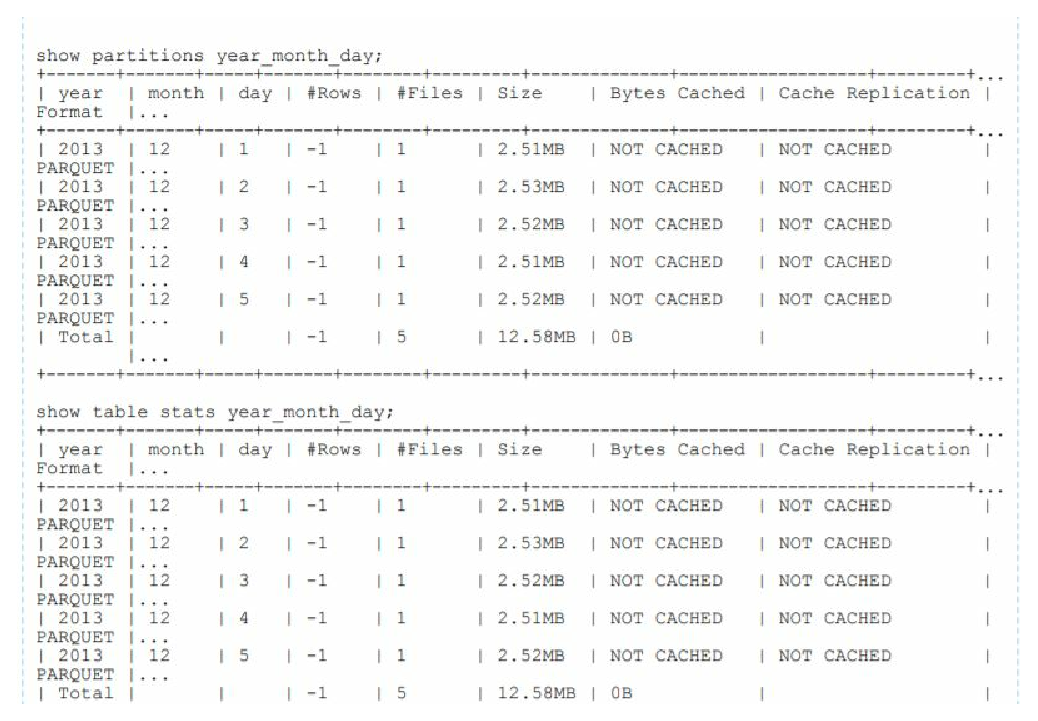
\includegraphics[width=\linewidth, height=4in, keepaspectratio]{StatFig1.eps}
\end{figure}

In addition to whole table statistics, statistics gathered on a by-column basis are also useful for query optimization.
“This technique is most valuable for columns compared across tables in JOIN queries, to help estimate how many rows the query will retrieve from each table.”
The COMPUTE STATS command computes column statistics as well as full table statistics.
Column statistics can be seen using the SHOW COLUMN STATS command. 

\begin{center}
\begin{tabular}{ |c| }
    \hline
    SHOW COLUMN STATS table\_name; \\
    \hline
\end{tabular}
\end{center}

Unlike table statistics, partitioning does not affect column statistic gathering, because column statistics are only calculated for the entire table, not individual partitions.
However, an additional kind of statistics, called Incremental Statistics, can be gathered for partitioned tables. 

\begin{figure}[ht]
    \centering
    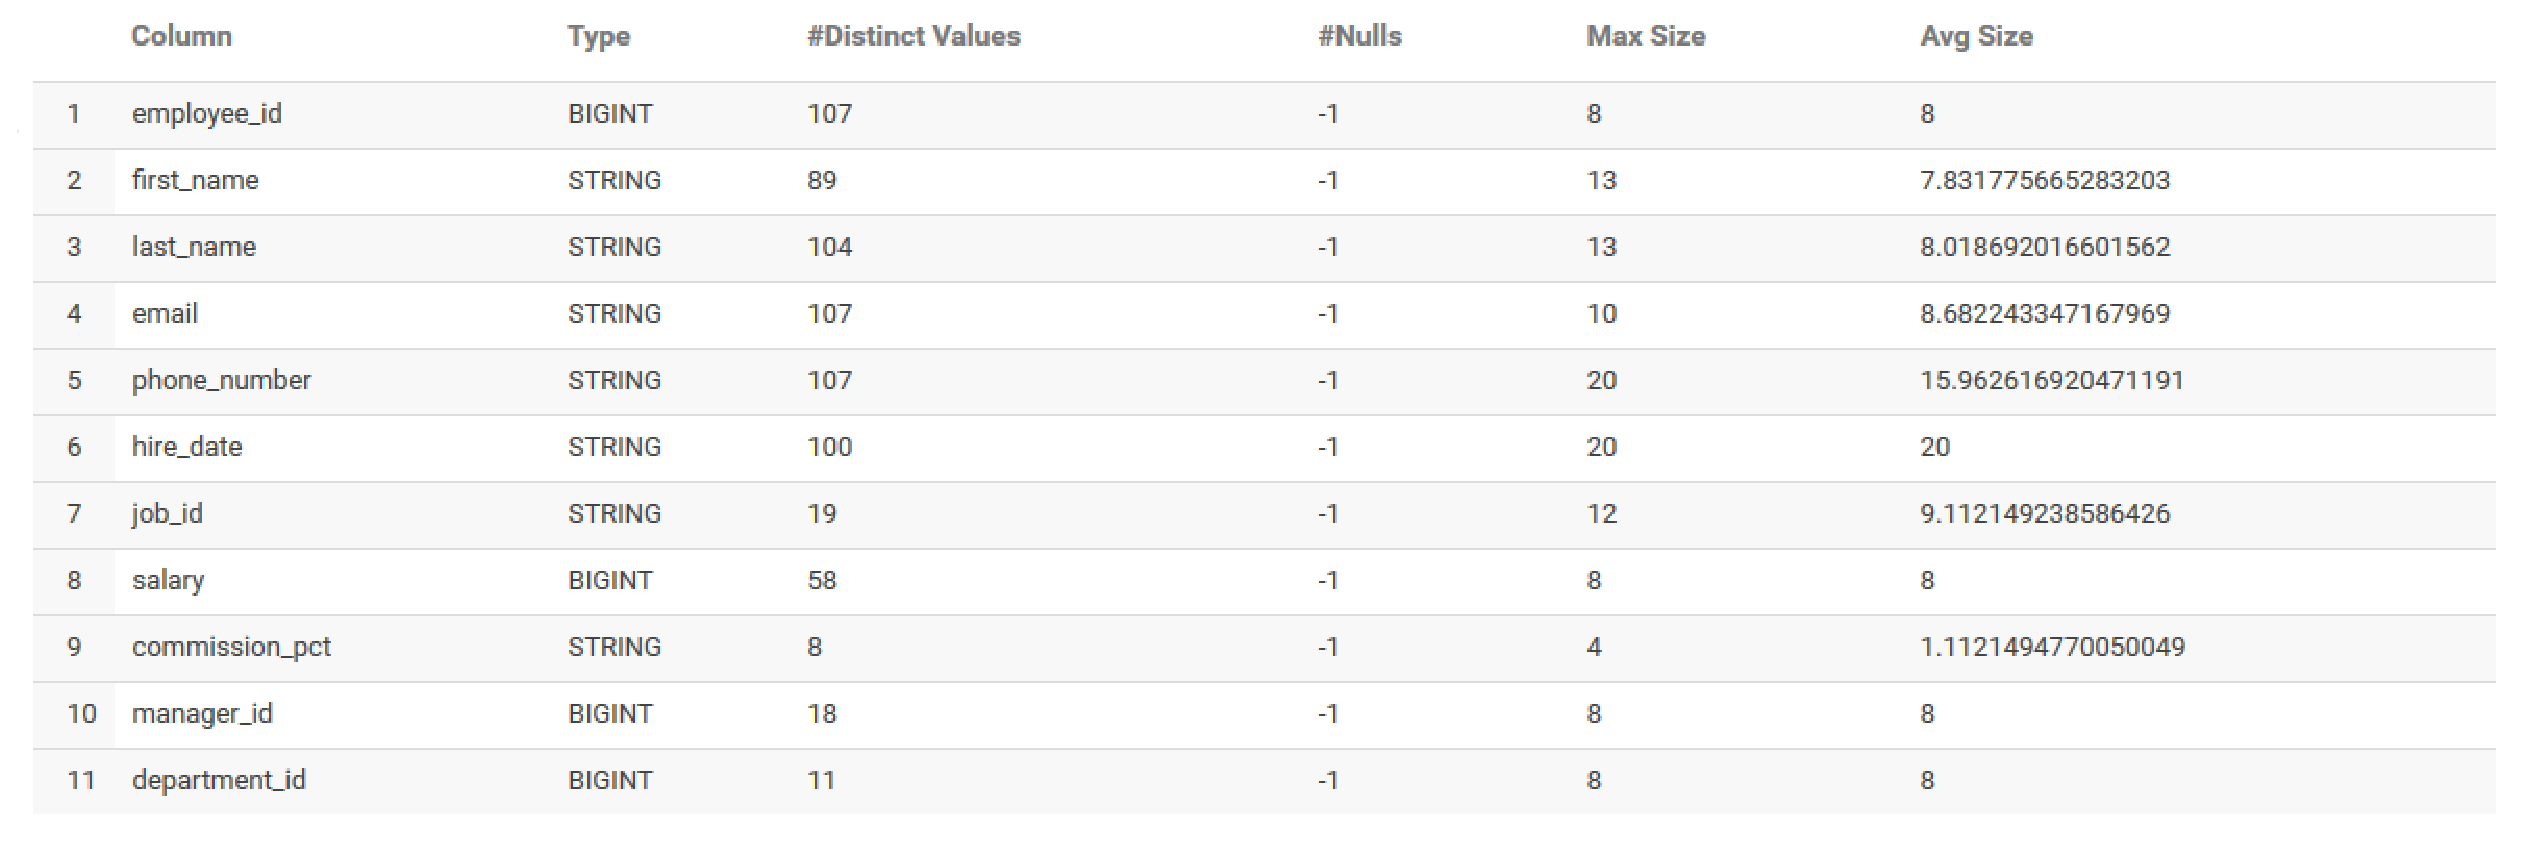
\includegraphics[width=\linewidth, height=4in, keepaspectratio]{ili0.eps}
\end{figure}

When you compute incremental statistics, statistics are only gathered for partitions that do not yet have incremental statistics. 
This way, statistics are only computed for newly added partitions, instead of for the entire table. 
This keeps statistics up to date without incurring the overhead of reprocessing the entire table each time data is added. 
They can be computed with the command:
\begin{center}
\begin{tabular}{ |c| }
    \hline
    COMPUTE INCREMENTAL STATS table\_name [Partition key]; \\
    \hline
\end{tabular}
\end{center}
Running the above command without a specified partition causes incremental stats to be computed for all partitions currently without incremental stats.
If it is the first time is it run, it will compute stats for the whole table. 
However, all future runs will only compute stats for new partitions. 
Due to this, computing incremental stats will take more time than the regular COMPUTE STATS command for the same volume of data, and so should not be used for regularly updating entire tables worth of statistics. 
Computing incremental stats also uses some memory in the catalogd process-- about 400 bytes of overhead memory for each column in a partition.
This memory is reserved in the catalogd daemon, the statestored daemon, and in each instance of the impalad daemon.

To maintain accurate statistics for each table, run your chosen COMPUTE STATS command every time new data is loaded into a table, and after the amount of data in a table is changed significantly, such as from an INSERT, add PARTITION, or LOAD DATA command. 
\newline
\newline

Manual Statistic Manipulation

There are many cases where manually manipulating table and column statistics is useful, including but not limited to:
\begin{enumerate}
    \item When running a full COMPUTE STATS command is not time efficient
    \item When the current metadata causes the Impala optimizer to choose an inefficient JOIN operation
    \item When adding data to a table which has less columns than the data 
    \item When importing a new table with which you wish to use the statistics of an existing table instead of computing new statistics
\end{enumerate}

In such cases, the metadata where table statistics are stored can be changed using an ALTER TABLE command. 

\begin{center}
\begin{tabular}{ |c| }
    \hline
    NOTE: Most ALTER TABLE commands effect table and column metadata ONLY. \\
    Commands do not affect the underlying datafiles. \\
    \hline
\end{tabular}
\end{center}

The most useful metadata to change will be the number of rows contained in a table. You can change the number of rows by table and by partition.
In the below example, we first set a table named table\_name’s number of rows to be 100, then we set a specific partition of table\_name, partitionP (partitioned based on ‘year’ and ‘month’) , number of rows to be 5. 
Remember, the ALTER TABLE command does not change the actual data,  just the metadata store. 
The datafile table\_name is stored in will still have its original number of rows after the command is run.

\begin{center}
\begin{tabular}{ |c| }
    \hline
    -- change the numRows property for whole table \\
    ALTER TABLE table\_name SET tblproperties( 'numRows' = '100', \\ 'STATS\_GENERATED\_VIA\_STATS\_TASK'='true'); \\

    -- change the numRows property for the partition \\
    ALTER TABLE table\_name partition(year=2009, month=4) \\
    SET tblproperties ('numRows'='5', 'STATS\_GENERATED\_VIA\_STATS\_TASK'='true'); \\
    \hline
\end{tabular}
\end{center}

In CDH 5.8 / Impala 2.6 and higher, you can append commands to ALTER TABLE to manipulate the statistic values of a specific column.
You can only set statistic values for the entire table’s columns. 
As of the writing of this paper,  you cannot set column statistics by partition.
You also can only alter statistic values for one column per command.
If you wish to set statistics for multiple columns, this must be done in separate commands. 

Changing statistics requires use of case-insensitive symbolic names for each statistics:
\begin{center}
\begin{tabular}{ |c|c| }
    \hline
    Statistic Name & Symbolic Name \\
    \hline
    Number of Distinct Values & numDVs \\ 
    \hline
    Average Size of Data & avgSize \\
    \hline
    Maximum Size of Data & maxSize \\
    \hline
\end{tabular}
\end{center}

To change these statistics using the SET COLUMN STATS command, both the symbolic (key) names and their new values must be quoted as in the examples below.

\begin{center}
    \begin{tabular}{|c|}
    \hline
    -- Create table with 1 column \\
    CREATE TABLE t1 (x int); \\
    INSERT INTO t1 VALUES (1), (2); \\ 

    -- Alter table to contain 2 more columns, insert data with 3 columns \\ 
    ALTER TABLE  t1 ADD COLUMNS (s string, t timestamp); \\
    INSERT INTO t1 VALUES (3, 'three', now()); \\

    -- Alter table to contain 1 more column, insert data with 4 columns \\
    ALTER TABLE t1 ADD COLUMNS (b boolean); \\
    INSERT INTO t1 VALUES (4, 'four', now(), true); \\

    -- All rows which existed before a column was added contain NULL for those columns \\
    SELECT * FROM t1; \\
    \hline
    \end{tabular}
\end{center}
\begin{figure}[ht]
    \centering
    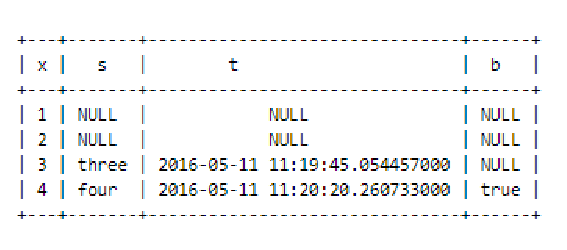
\includegraphics[keepaspectratio]{ili1.eps}
\end{figure}

\begin{center}
    \begin{tabular}{|c|}
    \hline
-- Drop column b, safe\\
ALTER TABLE t1 DROP COLUMN b;\\
SELECT * FROM t1;\\
    \hline
    \end{tabular}
\end{center}
\begin{figure}[ht]
    \centering
    
\includegraphics[keepaspectratio]{ili2.eps}
\end{figure}
\begin{center}
    \begin{tabular}{|c|}
    \hline
-- Drop inner column s, unsafe \\
-- Notice how Impala still reads the first and second columns from the datafile \\
-- Data from the former column s is now interpreted as data for column t \\
-- Depending on the underlying datafile, this could induce a conversion error,
-- because s’s datatype was Strings, \\
-- while t’s datatype is Timestamps \\
ALTER TABLE t1 DROP COLUMN s;\\
SELECT * FROM t1;\\
    \hline
    \end{tabular}
\end{center}

\begin{figure}[ht]
    \centering
    
\includegraphics[keepaspectratio]{ili3.eps}
\end{figure}

SQL Hints 

Impala supports SQL hint inclusion in queries with a similar syntax to SQL hints in Oracle systems.
Hints are suggestions or directives sent to the query optimizer to change its normal decision making process. 
They are most often used for resource-intensive queries--  such as JOINs between large tables where data is located across several nodes-- where an inefficient query plan can cause resource hogging and slow downs. 

Hints are specified in comments, using either  /* */ or -- notation, with a + symbol added before the hint name.
For example, the below code snippets showing JOIN hints are equivalent:
\begin{center}
\begin{tabular}{ |c| }
    \hline
    SELECT STRAIGHT\_JOIN clause FROM \\
    table\_Name1 \\
    JOIN  /* +SHUFFLE | BROADCAST */ \\
    table\_Name2; \\
    ------------------------------------ \\
    SELECT STRAIGHT\_JOIN clause FROM \\
    table\_Name1 \\
    JOIN  -- +SHUFFLE | BROADCAST \\
    table\_Name2;     \\
    \hline
\end{tabular}
\end{center}

The SHUFFLE and BROADCAST hints change the execution of join queries.
Other types of queries that support sql hints are INSERT-SELECT, CREATE TABLE AS SELECT.

The main JOIN sql hints are SHUFFLE leads to a “partitioned” join strategy, which divides up the corresponding rows from both tables and sends those subsets of the rows to other nodes for processing.
It is recommended when you are joining two large tables of relatively the same size, both of which have table statistics computed.
In contrast, BROADCAST sends the entire right-hand table to all nodes involved in processing the join.
It is the default join type used when statistics are unavailable, but is otherwise only recommended when joining a table with a significantly smaller right-hand table. 

\subsubsection{Amy Tang}
File Formats

The choice of data structure is an important decision that influences the performance, stability and accessibility.
Tabular data are inherently rectangular.
More strictly, every row has the same set of column nodes and every record share same variables.
In contrast, columnar storage stores data in columns.
The database can then access the data more precisely and prevent from scanning the unwanted data in row.
This structure can efficiently write and read data from storage disk.
Dremel and Solar are two successful distributed system that implement shared everything architecture with columnar data structure.
According to the Dremel paper, it claims that columnar- nested data structure help their shared disk system access data faster and reduce CPU cost due to cheaper compression \cite{Dremel}.
On the other hand, Solar used the share everything architecture base on tree data set.
They increase the performance and scalability by adding storage nodes that are used for data storage and read access \cite{zhu2018solar}.  

Impala supports several file formats that used in Apache Hadoop.
Impala can also load and query data from different files produced by Pig or Hive.
It is important to choose file format used in Impala table since file format has significant impacts on the performance.
For example, some file formats enable compression that may affect size of data and consequently lead to I/O and CPU resources required to deserialize data.
With this advantage, it can limit the query performance since querying often involves decompressing data.
To reduce the data transfer time from disk to memory, compressing data can bring a smaller number of data to being processed.
Some file formats are structured, which included metadata and built-in compression.
File formats supported in Impala are: Parquet, Avro, Text, RCFile, and SequenceFile.
On the other hand Avro , Parquet and Optimized Row Columnar (ORC) are three optimized file formats that used in Hadoop clusters.
Each of these file formats are unique and have their own relative advantages and disadvantages.  

Parquet

Parquet is a column-oriented file format. In contrast to row-oriented approach, it is more efficient for storage and performance. The values of each columns are organized and adjacent, so that it enables better compression. Since that, Parquet is a good choice when you need to query a specific column with wide table, or work on some aggregation operations such as SUM() and AVG() that need to process most of the values in a column. Parquet table can minimize I/O by reading less data and retrieve values from column quickly, and thus improve the performance because the I/O cost may strongly  influenced by the number of columns needed to be processed. On the other hand, some complex types such as ARRAY, STRUCT and MAP are currently supported only by the Parquet file format. 

When you try to load data that is already in the Impala or Hive table into Parquet table, even if the data is in a different file format or partitioning scheme, you can easily use the Impala INSERT...SELECT syntax.
The block size is the number of segments which hold columns entries in the Parquet file. 
For Parquet table, INSERT statement  requires space in the HDFS to write one block, and its default block size is 1 GB.
If the HDFS does not have enough space, an INSERT might fail.
When the system fail to INSERT into a partitioned table due to lack of the capacity, you can use hint keyword [SHUFFLE] or [NOSHUFFLE] (including the square brackets) before the SELECT keyword and after the PARTITION clause.
[SHUFFLE] reduces overall resource usage by select the query plan that has the minimized number of files being written into HDFS.
[NOSHUFFLE] may bring to an insertion failure as well because it select a faster query plan and sometime create large number of small data, so it is not recommended.
Impala will choose use or not to use the hint depends on the number of values in columns and the number of nodes that going to be process in the INSERT operation. 

Avro

Avro is a row major file format. 
Impala can query and create Avro tables, but not insert to them. 
For insertion, you can use Hive to accomplish and switch back to Impala.
LOAD DATA can be used in both Avro and Impala if there already have Avro data file.
Impala can move it to the Avro table but not create new Avro data file.
Avro schemas are defined with JSON and so it stores data definition in JSON after creating Avro tables.
Currently, Avro tables does not support TIMESTAMP columns.
There are two functions that help to store time values: UNIX\_TIMESTAMP() or EXTRACT(). UNIX\_TIMESTAMP() convert the STRING type of values into BIGINT type, and EXTRACT() create separate columns for date and time fields.

For some reason, mismatch of values type may occured between Avro schema and column definition in the database.
To solve this problem, Impala uses schema reconciliation to check mismatching number of columns.
Impala will choose to use the definition in Avro schema when there is mismatch in number of column, column name and column type.
For the restriction mentioned above, a TIMESTAMP definition in Impala maps to Avro STRING, which is a representation in the Avro schema.
Moreover, Avro supports schema evolution to handle old and new schema. Meanwhile, people can work with different version of schema at the same time.

ORC

Optimized Row Columnar (ORC) stores data in column format.
To be more specific, it stores collections of rows data into a columnar layout. This enables parallel processing for row collections.
Each row data is called stripe. In a stripe, it contain index data, row data that is used in table scan and stripe footer.
At the end of the file has file footer and postscript to store some information such as numbers of rows, compression parameter and column-level aggregate min, max, sum and count. 



\nocite{*}
\bibliographystyle{IEEEtran}
\bibliography{references}

\end{document}
